\documentclass[a4paper, article, oneside, UKenglish]{memoir}


%% Title page
\usepackage{projectfp} % [MAT2000], [MAT2500], [MEK3200] or [STK-MAT2011]


%% Encoding
\usepackage[utf8]{inputenx} % Source code
\usepackage[T1]{fontenc}    % PDF


%% Fonts and typography
\usepackage{lmodern}           % Latin Modern Roman
\usepackage[scaled]{beramono}  % Bera Mono (Bitstream Vera Sans Mono)
\renewcommand{\sfdefault}{phv} % Helvetica
\usepackage[final]{microtype}  % Improved typography
\renewcommand{\abstractnamefont}{\sffamily\bfseries}                 % Abstract
\renewcommand*{\chaptitlefont}{\Large\bfseries\sffamily\raggedright} % Chapter
\setsecheadstyle{\large\bfseries\sffamily\raggedright}               % Section
\setsubsecheadstyle{\large\bfseries\sffamily\raggedright}            % Subsection
\setsubsubsecheadstyle{\normalsize\bfseries\sffamily\raggedright}    % Subsubsection
\setparaheadstyle{\normalsize\bfseries\sffamily\raggedright}         % Paragraph
\setsubparaheadstyle{\normalsize\bfseries\sffamily\raggedright}      % Subparagraph

%% Mathematics
\usepackage{amssymb}   % Extra symbols
\usepackage{amsthm}    % Theorem-like environments
\usepackage{thmtools}  % Theorem-like environments
\usepackage{mathtools} % Fonts and environments for mathematical formuale
\usepackage{mathrsfs}  % Script font with \mathscr{}


%% Miscellaneous
\usepackage{graphicx}  % Tool for images
\graphicspath{{figures/}}
\usepackage{babel}     % Automatic translations
\usepackage{csquotes}  % Quotes
\usepackage{textcomp}  % Extra symbols
\usepackage{listings}  % Typesetting code
\lstset{basicstyle = \ttfamily, frame = tb}


%% Bibliography
\usepackage{mathscinet}
\usepackage[backend    = biber,
            sortcites  = true,
            giveninits = true,
            doi        = false,
            isbn       = false,
            url        = false,
            sortlocale = nb_NO,
            style      = alphabetic]{biblatex}
\DeclareNameAlias{sortname}{family-given}
\DeclareNameAlias{default}{family-given}
\DeclareFieldFormat[article]{volume}{\bibstring{jourvol}\addnbspace#1}
\DeclareFieldFormat[article]{number}{\bibstring{number}\addnbspace#1}
\renewbibmacro*{volume+number+eid}
{
    \printfield{volume}
    \setunit{\addcomma\space}
    \printfield{number}
    \setunit{\addcomma\space}
    \printfield{eid}
}
\addbibresource{bibliography.bib}


%% Cross references
\usepackage{varioref}
\usepackage[pdfusetitle]{hyperref}
\urlstyle{sf}
\usepackage[nameinlink, capitalize, noabbrev]{cleveref}
\crefname{chapter}{Section}{Sections}


%% Theorem-like environments
\declaretheorem[style = plain, numberwithin = chapter]{theorem}
\declaretheorem[style = plain,      sibling = theorem]{corollary}
\declaretheorem[style = plain,      sibling = theorem]{lemma}
\declaretheorem[style = plain,      sibling = theorem]{proposition}
\declaretheorem[style = definition, sibling = theorem]{definition}
\declaretheorem[style = definition, sibling = theorem]{example}
\declaretheorem[style = remark,    numbered = no]{remark}


%% Delimiters
\DeclarePairedDelimiter{\p}{\lparen}{\rparen}   % Parenthesis
\DeclarePairedDelimiter{\set}{\lbrace}{\rbrace} % Set
\DeclarePairedDelimiter{\abs}{\lvert}{\rvert}   % Absolute value
\DeclarePairedDelimiter{\norm}{\lVert}{\rVert}  % Norm


%% Operators
\newcommand{\diff}{\mathop{}\!\mathrm{d}}
\DeclareMathOperator{\im}{im}
\DeclareMathOperator{\rank}{rank}
\DeclareMathOperator{\E}{E}
\DeclareMathOperator{\Var}{Var}
\DeclareMathOperator{\Cov}{Cov}


%% New commands for sets
\newcommand{\N}{\mathbb{N}}   % Natural numbers
\newcommand{\Z}{\mathbb{Z}}   % Integers
\newcommand{\Q}{\mathbb{Q}}   % Rational numbers
\newcommand{\R}{\mathbb{R}}   % Real numbers
\newcommand{\C}{\mathbb{C}}   % Complex numbers
\newcommand{\A}{\mathbb{A}}   % Affine space
\renewcommand{\P}{\mathbb{P}} % Projective space


%% New commands for vectors
\renewcommand{\a}{\mathbf{a}}
\renewcommand{\b}{\mathbf{b}}
\renewcommand{\c}{\mathbf{c}}
\renewcommand{\v}{\mathbf{v}}
\newcommand{\w}{\mathbf{w}}
\newcommand{\x}{\mathbf{x}}
\newcommand{\y}{\mathbf{y}}
\newcommand{\z}{\mathbf{z}}
\newcommand{\0}{\mathbf{0}}
\newcommand{\1}{\mathbf{1}}


%% Miscellaneous
\renewcommand{\qedsymbol}{\(\blacksquare\)}


\title{Fire Detection Using MODIS}
\author{Paulina Tedesco}
%\supervisor{}
% Multiple supervisors: \supervisor{Supervisor 1}{Supervisor 2}...{Supervisor n}
% Skip supervisor for MAT2500


\begin{document}


\projectfrontpage


\begin{abstract}
    \noindent
    Brief summary of the paper.
\end{abstract}

% ------------------------------------------------------------------------------------------------------
\chapter{Introduction}

Wildfires are unplanned fires that occur in natural areas such as forests, grasslands, or prairies, causing a tremendous impact on the environment. They pose a threat to natural resources, properties, human health, wildlife, ecosystems, weather, and climate. 

Wildfire activity is strongly influenced by climate and weather conditions, and as global temperatures, droughts, and extremes increase, there appears to be an increasing trend in fire activity (\cite{jolly_and_william_2015}, IPCC). Two crucial factors that affect fires are high temperatures and low humidity. The main natural cause of fires is lightning, which is related to deep convective systems favored by warm conditions (\cite{veraverbeke_et_al_2017}). However, hotter and dryer conditions also set the stage for fires originated by human activity. Another consequence of a warmer climate is that nighttime temperatures are higher, allowing fires to burn at night and extending over more days, where, previously, cooler temperatures at night would weaken or extinguish the fires.

Fire feedbacks are complex mechanisms; fires can, directly and indirectly, increase carbon emissions to the atmosphere. While burning, they release carbon from trees or the soil. In addition, dead trees release carbon as they decompose and can no longer act as a carbon sink. There is also a mixed effect of aerosols on climate due to fires: on the one hand, dark aerosols (black carbon) absorb heat from the sunlight in the atmosphere and darken the surfaces contributing to its melt, while on the other hand, light-colored aerosols may have the opposite effect. Aerosols may also make it harder for water droplets to form in the tropics (\cite{tosca_et_al_2012}). Overall, fire feedback mechanisms have an impact on both local temperatures and the water cycle.

Understanding the immediate and long-term effects of wildfires requires global datasets, such as satellite data, that allow us to detect fires, map their burned areas, and trace the smoke in the atmosphere.

The summer 2018 was historically warm and dry in Scandinavia as well as in many countries in the Northern Hemisphere. The result has been many and large fires in the forest, in particular, during July and August. The worst affected country is Sweden, at least 40 fires were registered the $17^{th}$ of July according to The Local Sweden (\cite{the_local_sweden}).

Blocking events associated with a weaker than normal jet stream led to severe heat waves and droughts across Europe in 2018. Temperature anomalies in July were all positive in Europe, and particularly high in Scandinavia (see Figure \ref{fig:temperature_anomalies}). This much warmer than normal conditions were reflected in many temperature records; several locations in the Arctic recorded temperatures of $30^{\circ}$ degrees or higher (NOAA). Figure \ref{fig:highest_temp} ranks the maximum temperatures registered in Europe since 1950. The darkest red boxes indicate a historical maximum, the bright red ones are for the second highest maximum temperature, and so on. The continent was also affected by very dry conditions, for instance, Norway received 55\% of its normal precipitation (Figure \ref{fig:precipitation_percent}) registering the second driest July since records began in 1900.

\begin{figure}
    \centering
    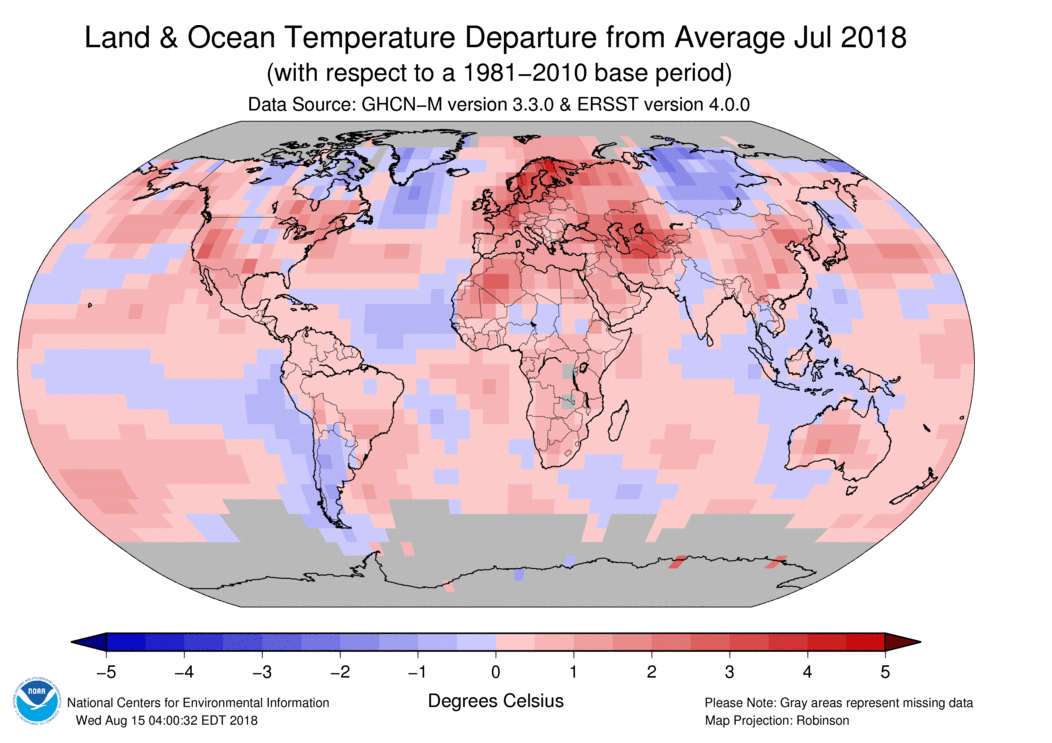
\includegraphics[scale=0.3]{NOAA/warm_anomalies.png}
    \caption{Global temperature anomalies in July 2018. Source: NOAA.}
    \label{fig:temperature_anomalies}
\end{figure}

\begin{figure}
    \centering
    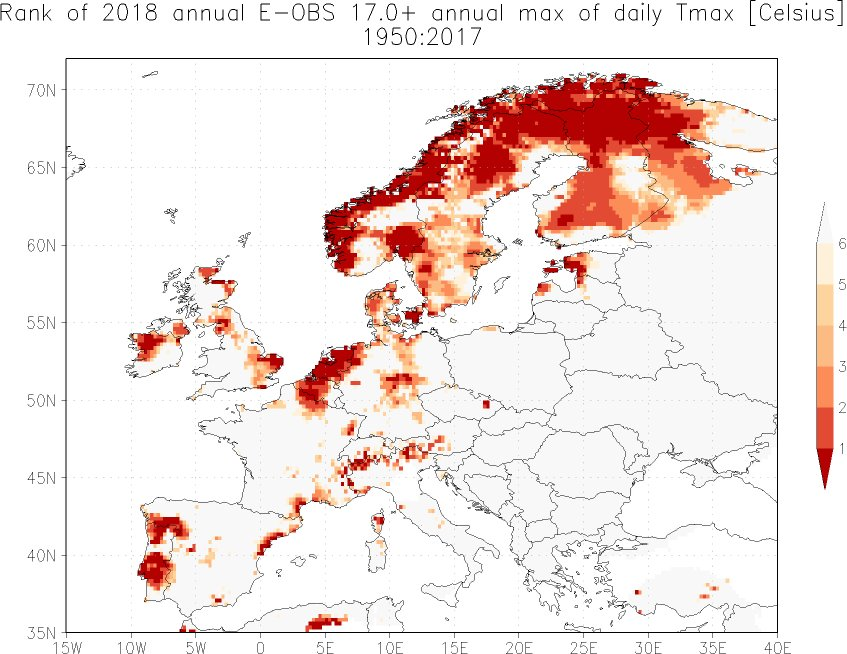
\includegraphics[scale=0.3]{NOAA/Highest_maximum_temperature_of_the_summer_2018_August_in_Europe.jpg}
    \caption{Highest maximum temperatures of the summer 2018 in Europe. Source: https://twitter.com/gjvoldenborgh/status/1026211064285995009}
    \label{fig:highest_temp}
\end{figure}

\begin{figure}
    \centering
    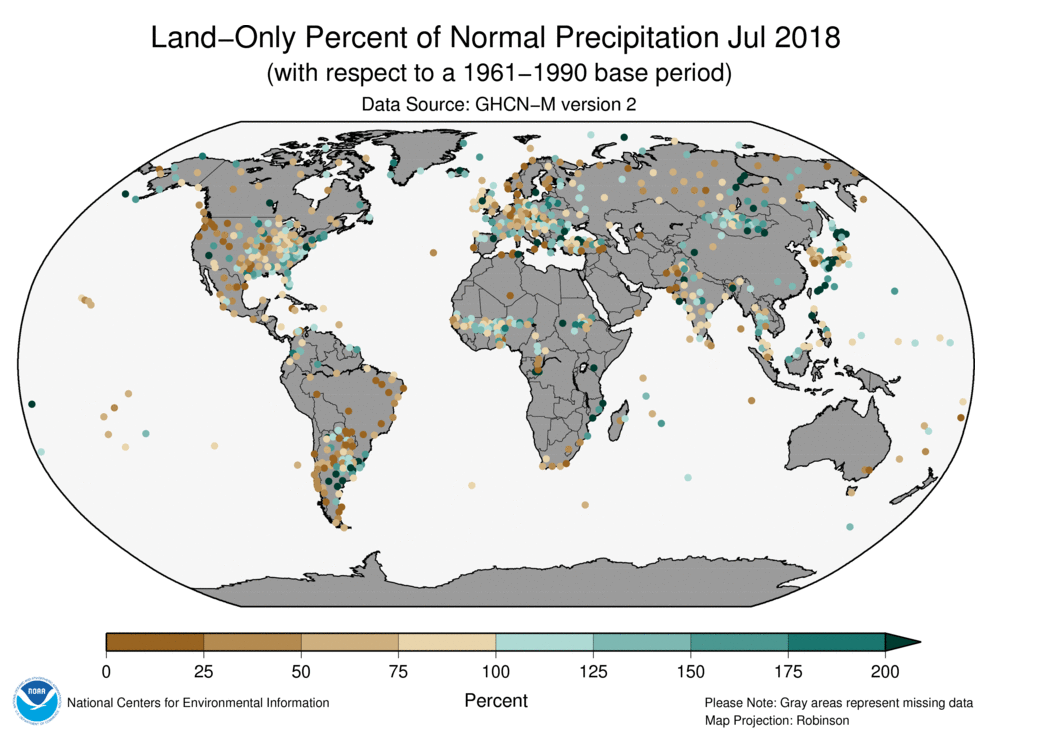
\includegraphics[scale=0.3]{NOAA/dry_anomalies.png}
    \caption{Global land percent of normal precipitation July 2018. Source: NOAA.}
    \label{fig:precipitation_percent}
\end{figure}

https://www-sciencedirect-com.ezproxy.uio.no/science/article/pii/S0379711218303941


% ------------------------------------------------------------------------------------------------------
\chapter{Methods and Data}

The method used to detect fires using MODIS data is described in \citeauthor{giglio_et_al_2016} (\citeyear{giglio_et_al_2016}), although the values of the threshold were modified taking into consideration the channels from MODIS used, that clouds are not filtered, and the total area affected by wildfires in Sweden as of July 23 (\cite{2018_sweden_wildfires}).

\subsection{Data}

Native brightness temperatures from two channels from the Collection 6 MODIS Level-1B radiance product aggregated to 1-km spatial resolution were used in this project. Channel 20 and channel 31 will be denoted as $T_4$ and $T_{11}$ respectively. The original methodology (\cite{giglio_et_al_2016}) uses data from channel 21, but here we have used channel 20 since it was already available in UiO's servers.

\begin{table}[htbp]
    \centering
    \begin{tabular}{@{}ccc@{}}
        \toprule
        \(\boldsymbol{}\) & \(\boldsymbol{Band}\) & \(\boldsymbol{Bandwidth}\)
        \\
        \midrule
        $T_4$     & 20   & 3.660 - 3.840 
        \\
        $T_{11}$    & 31   & 10.780 - 11.280
        \\
        \bottomrule
    \end{tabular}
    \caption{Summary of MODIS channels used. The bandwidth is in $(\mu m)$}
    \label{tab:modis_bands}
\end{table}


% ------------------------------------------------------------------------------------------------------
\chapter{Analysis}

% ------------------------------------------------------------------------------------------------------
\chapter{Conclusions}


Optional. Results, consequences, future work.

\cref{tab:numbers} lists some integers satisfying \cref{eq:pythagoras} of \cref{thm:pythagoras}.




\printbibliography


\end{document}